\chapter{Design}

\todo{Discuss LimitedLiterature (citation) - quote in findings}

\section{Gameplay Overview}
\todo[inline]{Maybe draw an example as this is a bit confusing}
The game provides a fairly straightforward experience from the user's point of view.
Conceptually, it is a card game, so I will describe it as such.
The game consists of three decks which I dub `in play', `out of play' and `reserve'. In addition to this, there are $n$ `pillars' - these are attributes of importance within the game story's context. Each of these has a minimum, maximum and current value.
The `in play' deck has a defined starting set of cards, with the `reserve deck' containing all others - `out of play' starts empty.
Both decks are shuffled at the start of the game, and each pillar has a predefined starting value.

The player draws and reads a card from the play deck, each one showing the following information:

\begin{itemize}
	\item Title
	\item Description
	\item Choice \#1 (`accept')
	\item Choice \#2 (`reject')
	\item Requirements to draw
\end{itemize}
Each choice on a card consists of text detailing the response, and the effects of the response. Effects are made up of two parts - pillar changes, and cards added/removed. Pillar changes specify amounts to add or remove from one or more pillars. Cards added/removed defines which cards should be moved between `out of play' and `reserve'.
Requirements to draw consists of conditions that the current pillar levels must satisfy in order for this card to be drawn.

After each choice made (turn), any cards in `out of play' the meet the current pillar requirements are moved to `in play', and any `in play' that do not are moved to `out of play'.

The game ends when any of the pillars fall to their minimum value.

\section{UI}

\subsection{Game}
As described above, the game sounds like a lot of effort on behalf of the player, having to sort and shuffle cards. Fortunately, this effort can be removed completely through work done by the computer. This leaves a simple game from the user perspective; users are presented with a card, make a choice, and get the next card.

This meant that the design for the game UI could also be simple. Figure \ref{fig:game_comp} shows my first design for this UI alongside the final product. Initially, I wasn't sure whether the pillars should be visible to the user, however after some testing it was clear that they were needed to provide the player with feedback as they played the game, so they were later added to the top of the screen.

\begin{figure}[!h]
	\centering
	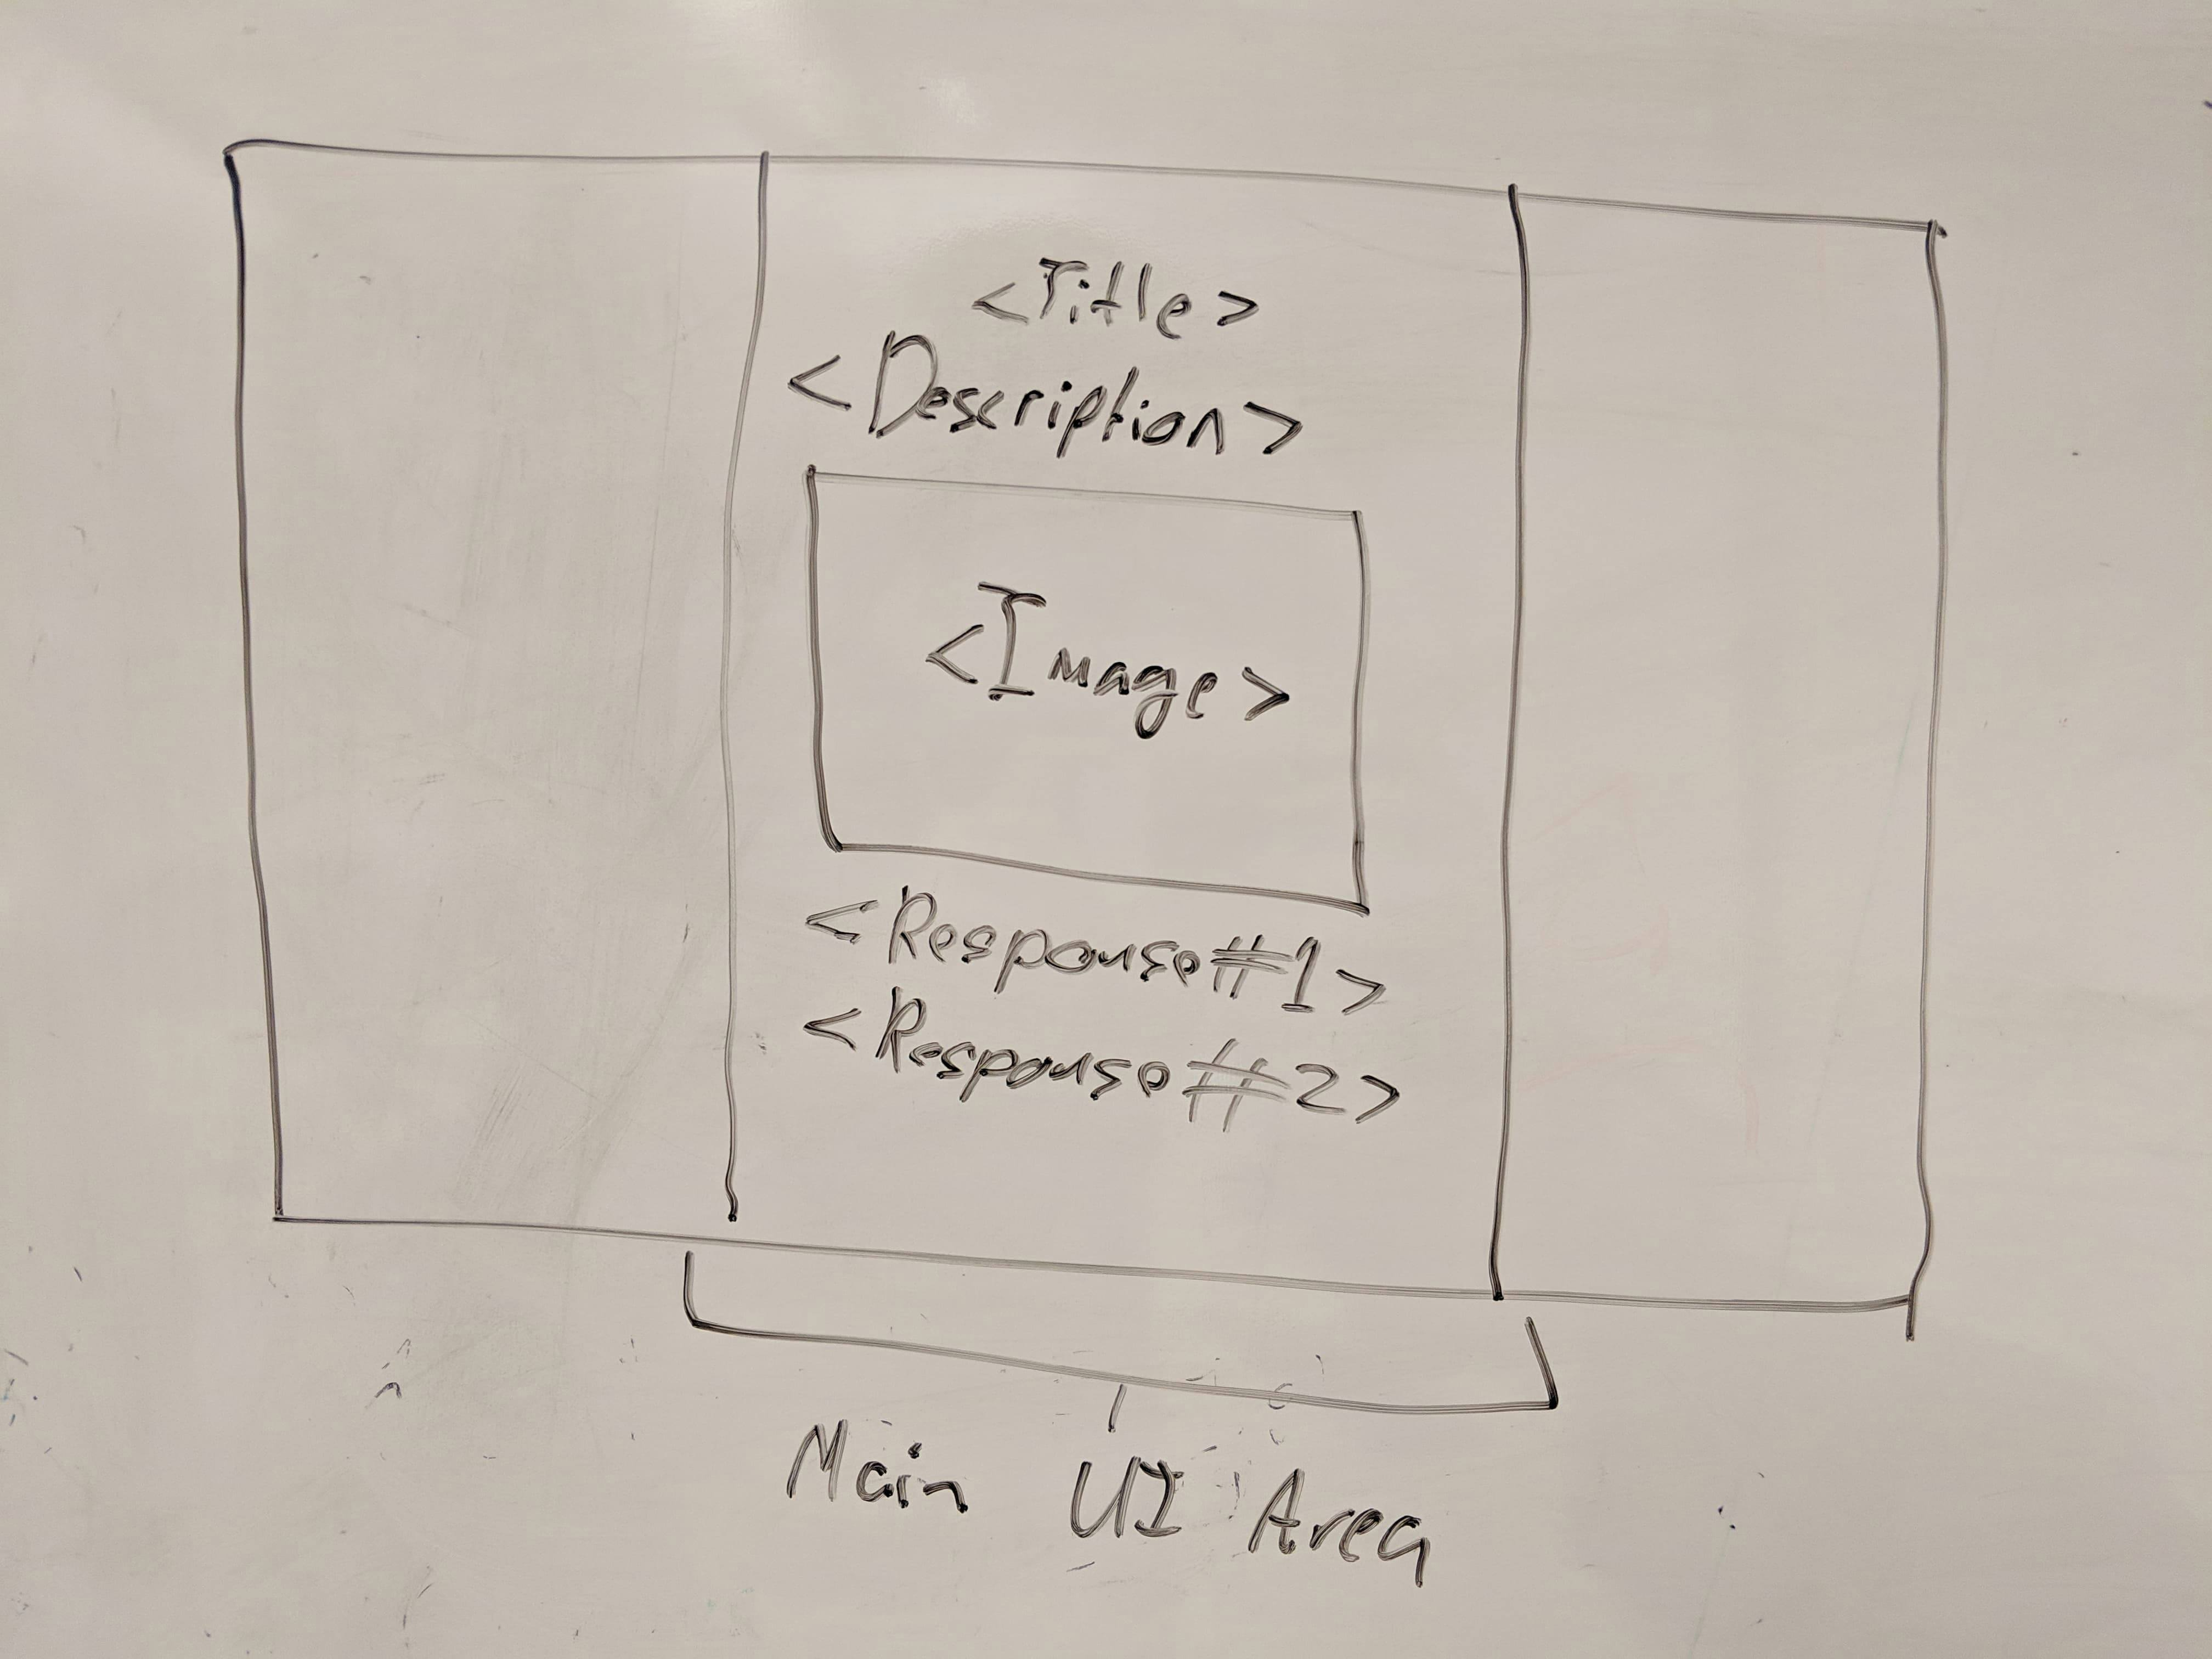
\includegraphics[width=0.36\textwidth]{./images/design/game_drawing.jpg}
	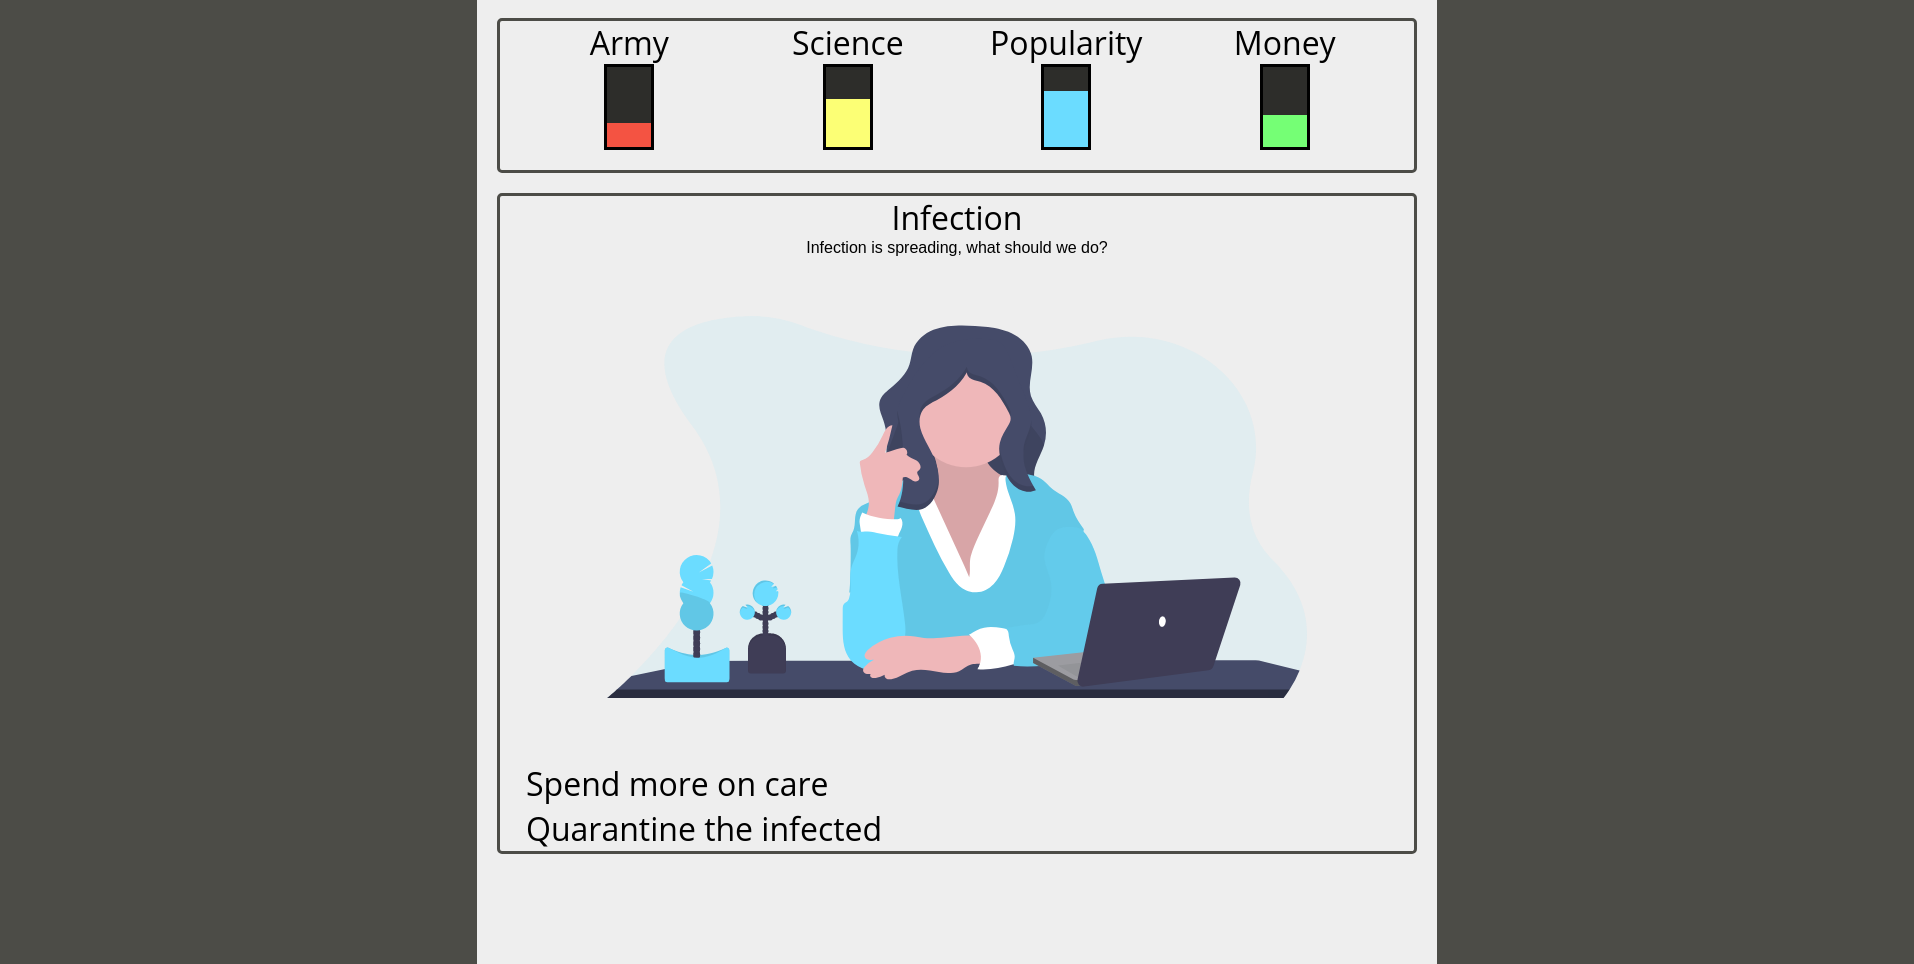
\includegraphics[width=0.54\textwidth]{./images/design/game.png}
	\caption{Comparison between initial and final designs for the game UI}
	\label{fig:game_comp}
\end{figure}

Pillars are displayed as vertical bars at the top of the screen, each having their own fill colour (customisable through game definition). I was inspired to add this colour customisation by other survey gamification tools, as a way to make the game more visually engaging, without forcing a colour scheme that could conflict with the desires of admin users. Pillars fill from bottom to top, and represent where the current value lies between the defined min and max.

\begin{figure}[!h]
	\centering
	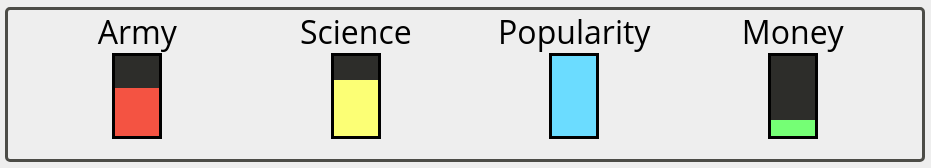
\includegraphics[width=0.9\textwidth]{./images/design/pillars.png}
	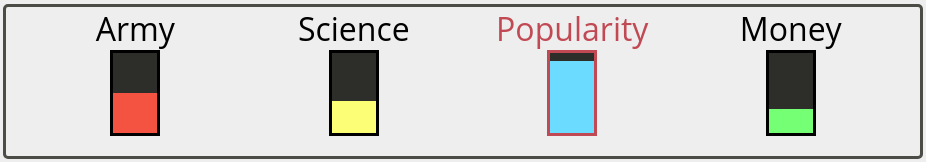
\includegraphics[width=0.9\textwidth]{./images/design/hover.png}
	\caption{Visualisation of a negative outcome; the red outline around \c{Popularity} }
	\label{fig:colour_comp}
\end{figure}

The image shown with a given card is dependent upon the pillars the card influences, as seen in figure \ref{fig:advisor_comp}. In this example game, I gave each pillar an `advisor' image, so that the advisor representing the pillar most affected by a card is shown.

\begin{figure}[!h]
	\centering
	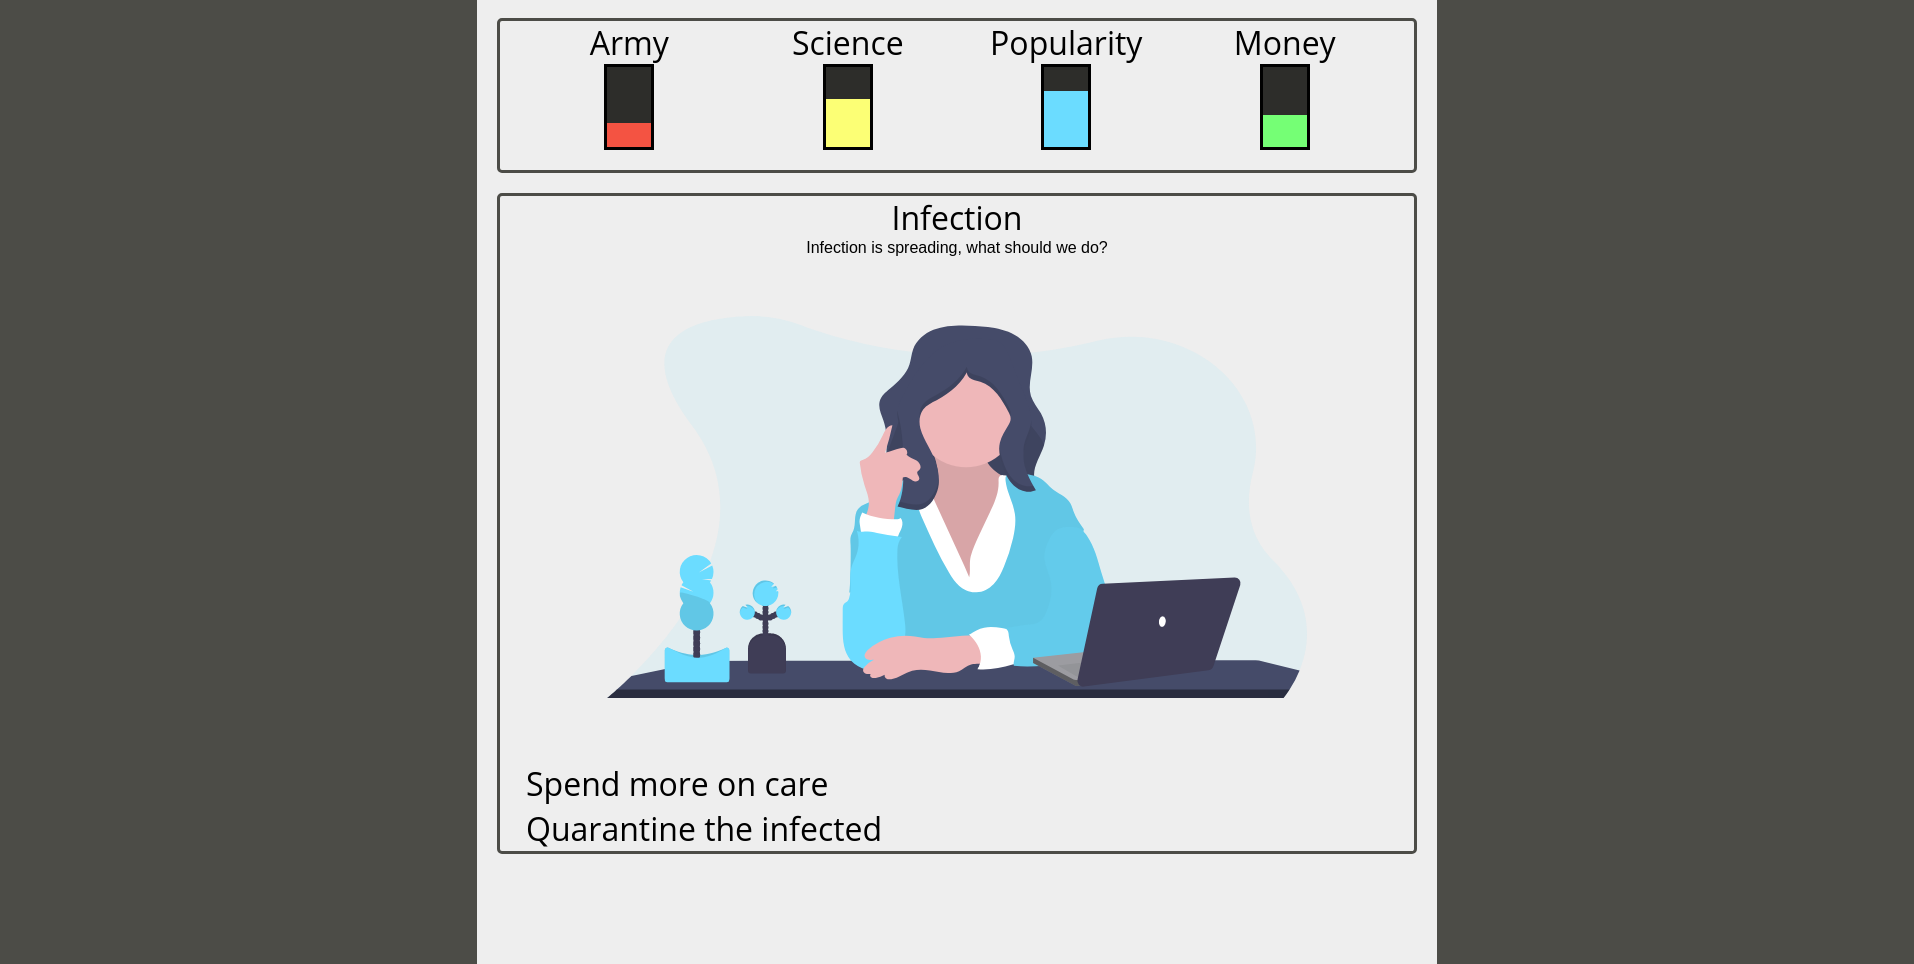
\includegraphics[width=0.45\textwidth]{./images/design/game.png}
	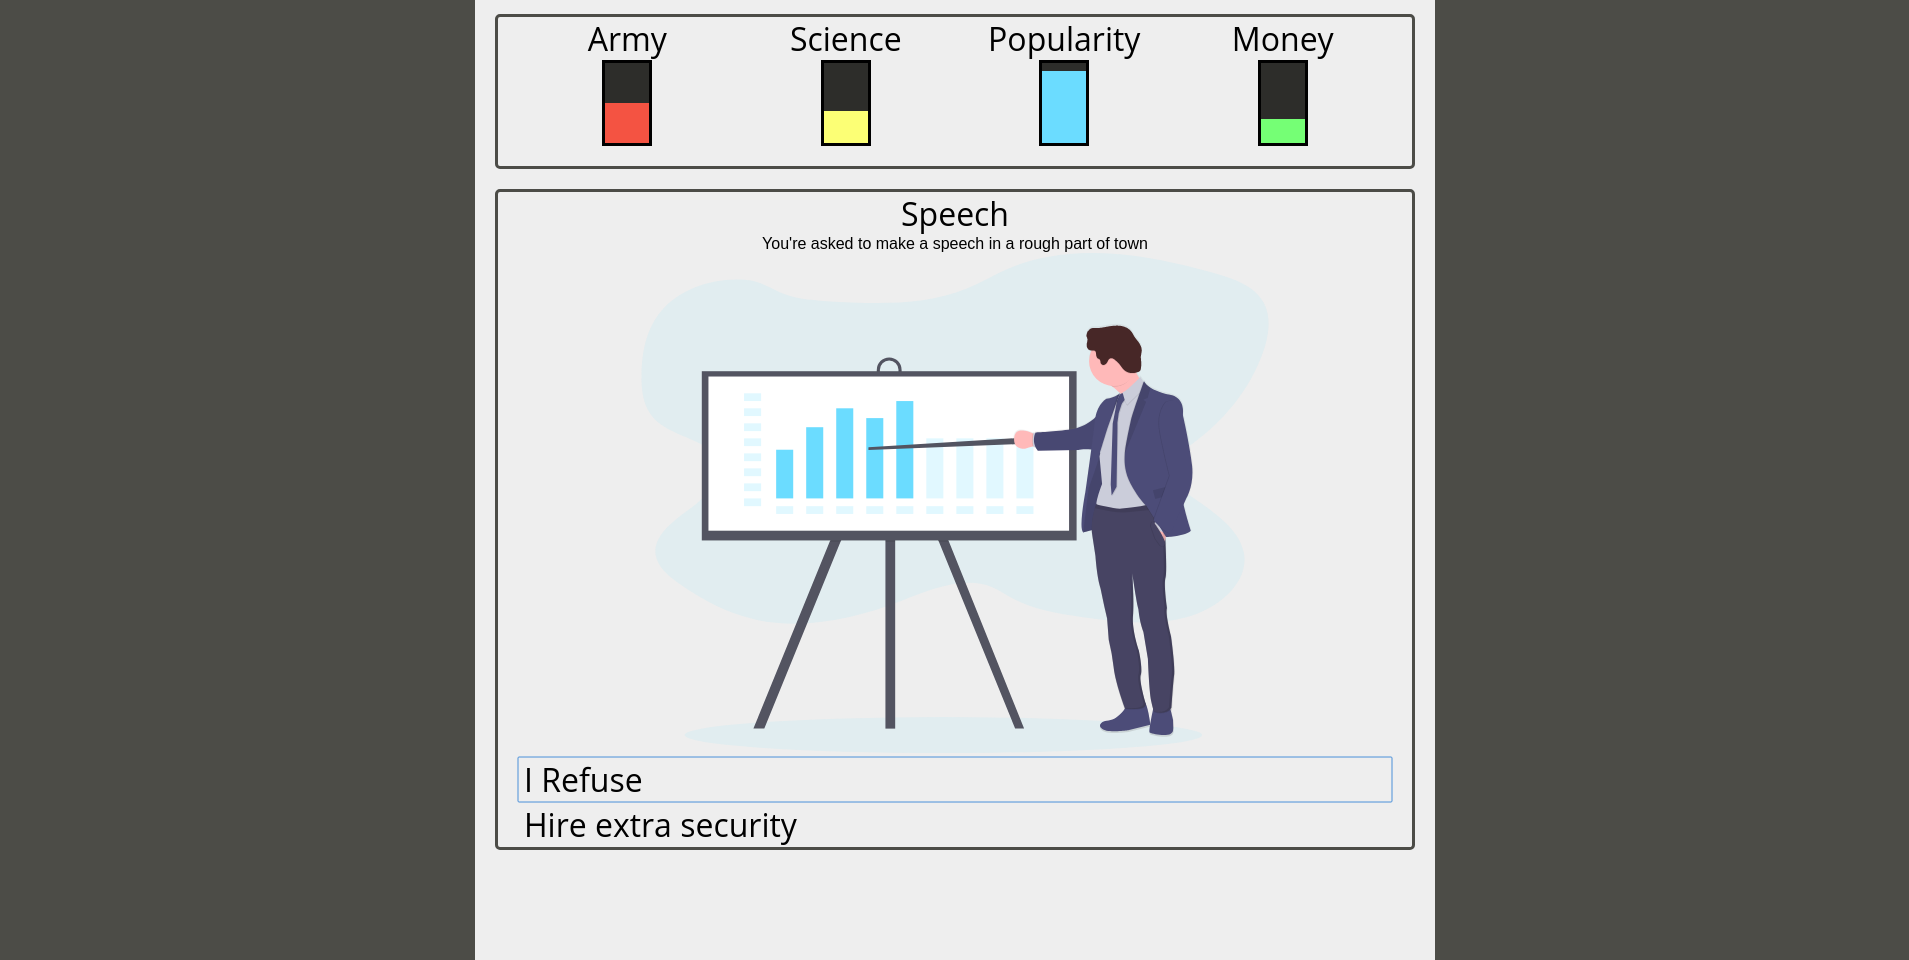
\includegraphics[width=0.45\textwidth]{./images/design/ecman_blue.png}
	\caption{These cards primarily affect different pillars, so they have different associated images}
	\label{fig:advisor_comp}
\end{figure}

As seen in figure \ref{fig:colour_comp}, not only can the image change, but the primary colour of the image may also change. I decided to include this feature as cards may affect more than one pillar, and this was not being represented when only using different images. With this colour shifting implemented, the image can represent secondary pillar effects.

\begin{figure}[!h]
	\centering
	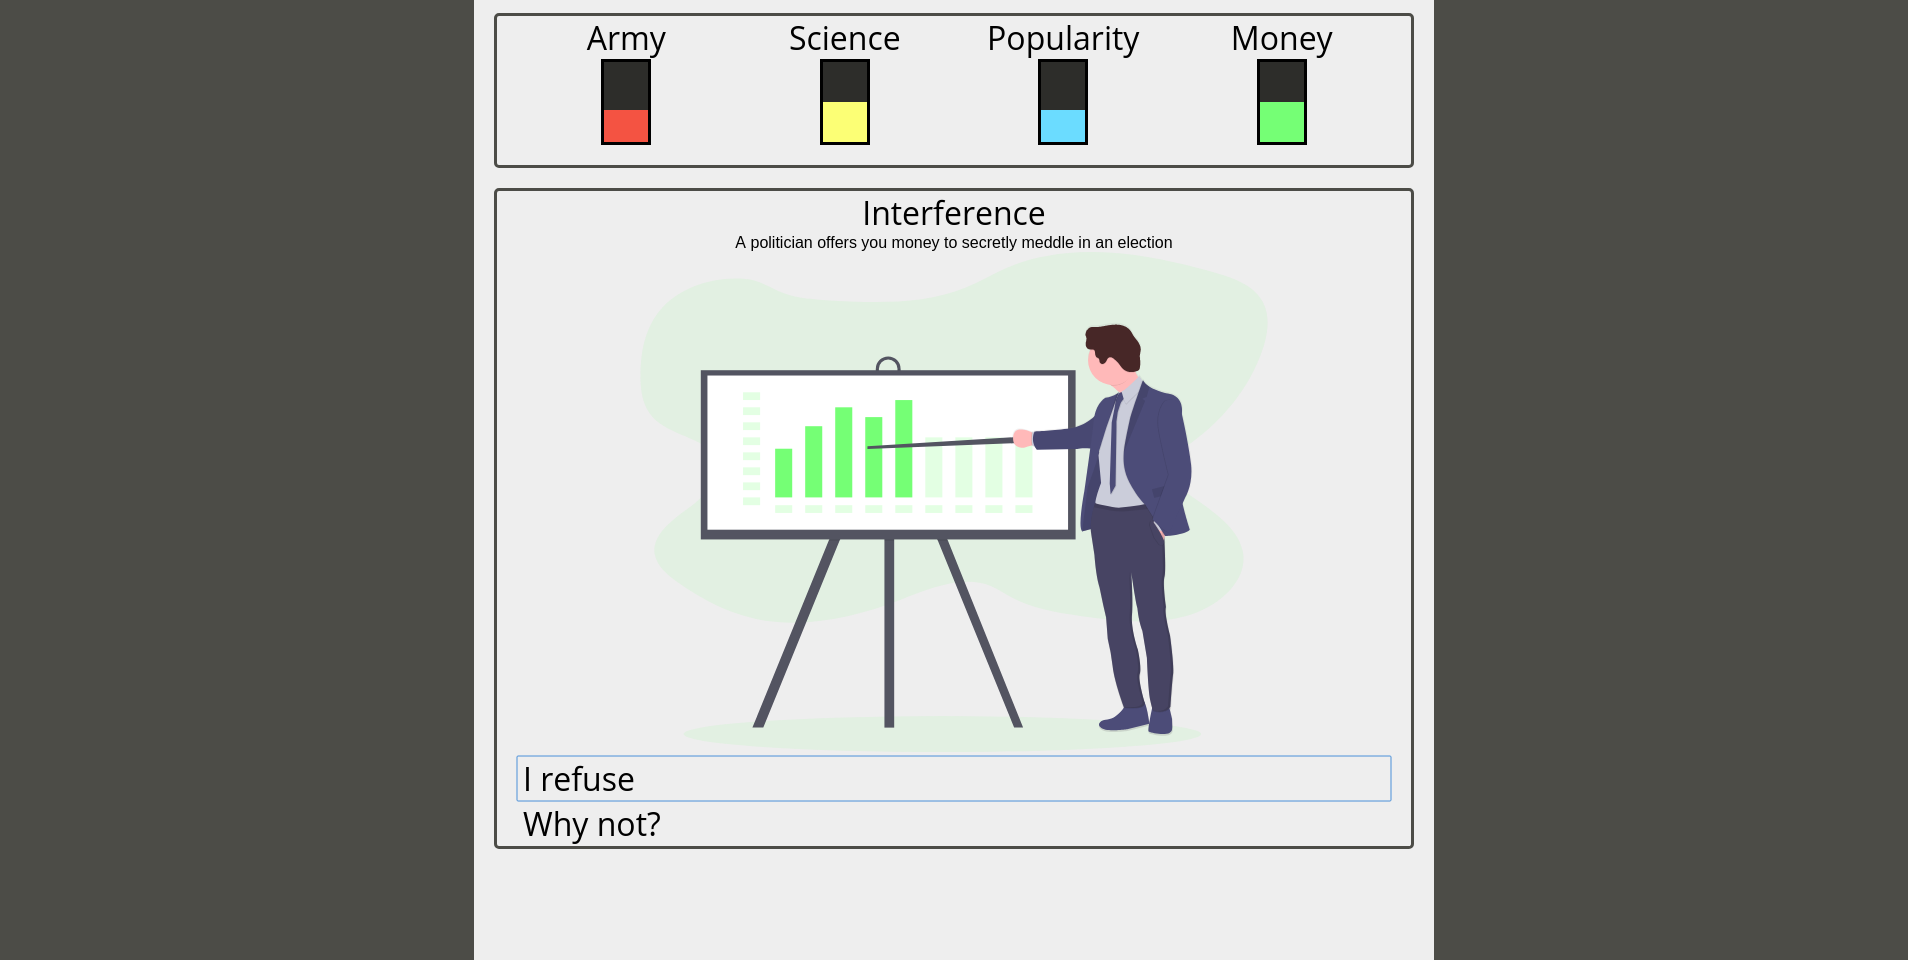
\includegraphics[width=0.45\textwidth]{./images/design/ecman_green.png}
	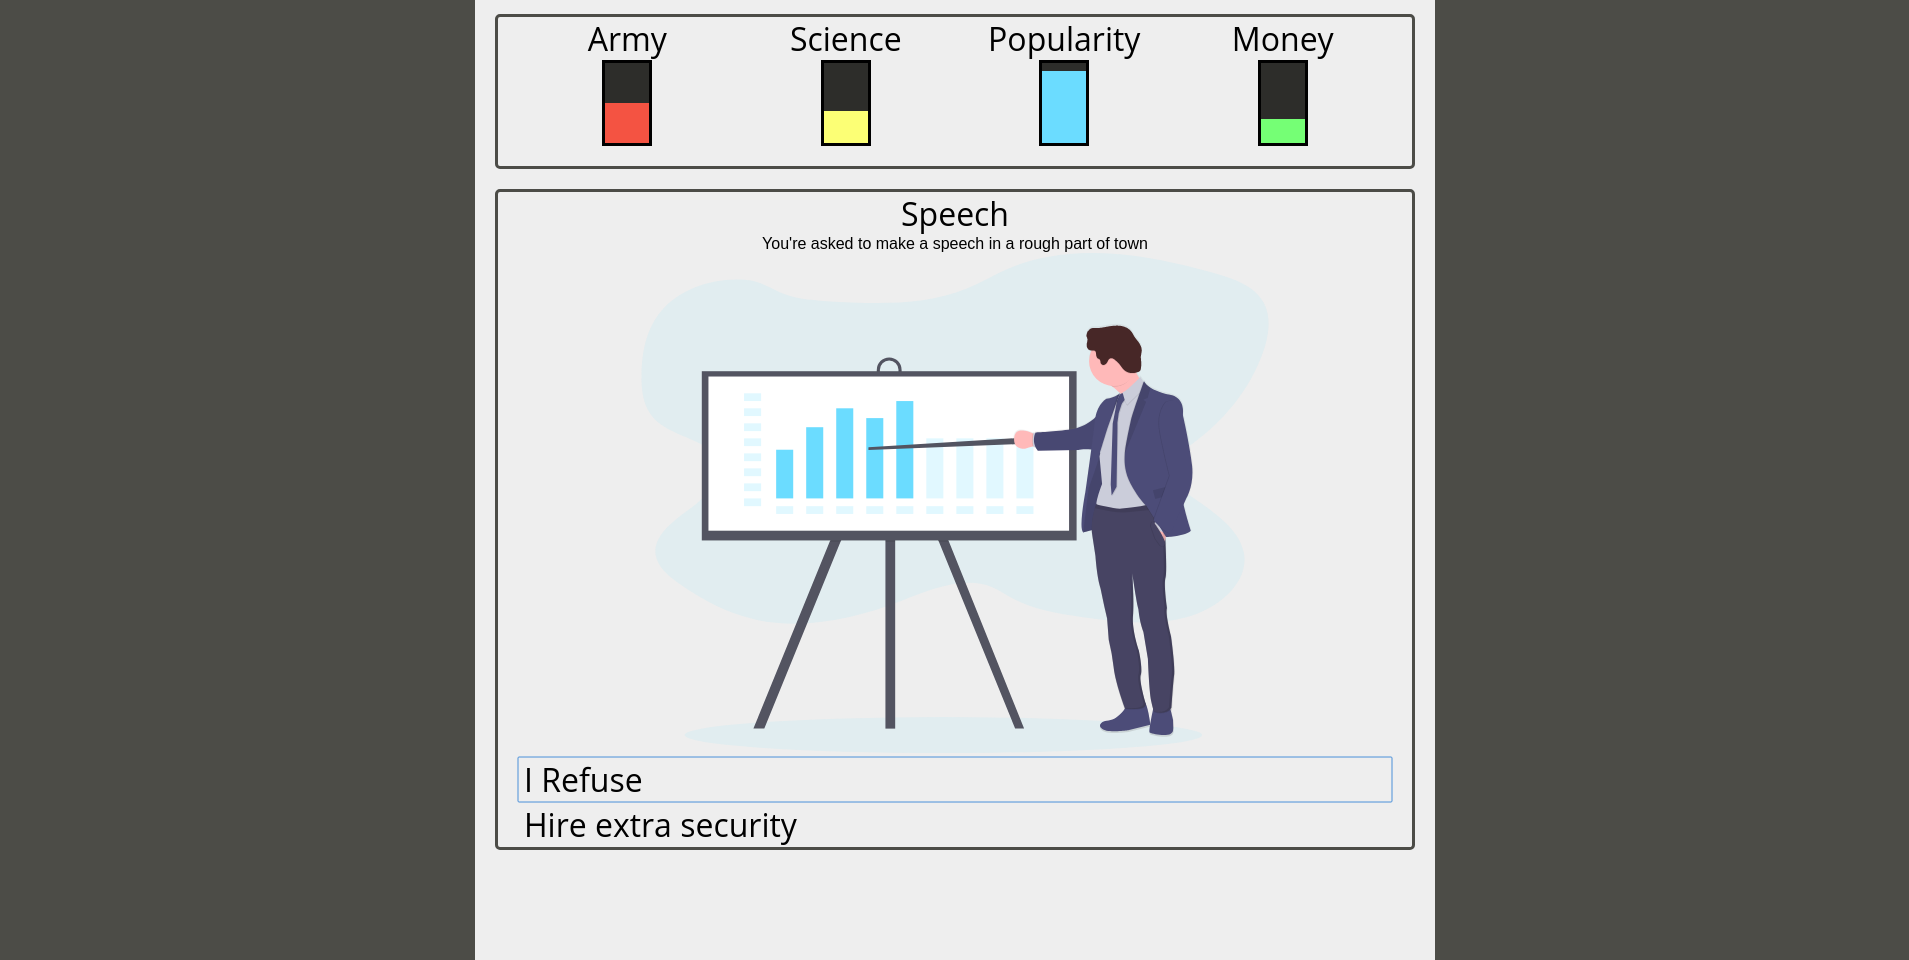
\includegraphics[width=0.45\textwidth]{./images/design/ecman_blue.png}
	\caption{Both of these cards primarily affect the \c{Money} pillar (they are being presented by the \c{Money} advisor) however the second also affects \c{Popularity}, so has a blue primary colour}
	\label{fig:colour_comp}
\end{figure}

\subsection{Admin tools}

\subsubsection{Game Maker}
The game maker interface was the most challenging to design, as I wanted the user to be able to maintain a high-level overview of the game while adding and editing pillars and cards.
After thinking this through, I initially settled on the design depicted in figure \ref{fig:game_maker}. The main theme is that editing is done in the left panel, while the right side continues to show an interactive view of the game, including a visualisation of the relationships between cards.
The final design ended up being roughly the same, however the card view is not as complex - connections between cards are not visualised, as after more consideration of the relationships involved, I could not think of a clear way to show this.
The cards are instead displayed in a grid in the final design.

\begin{figure}[!h]
	\centering
	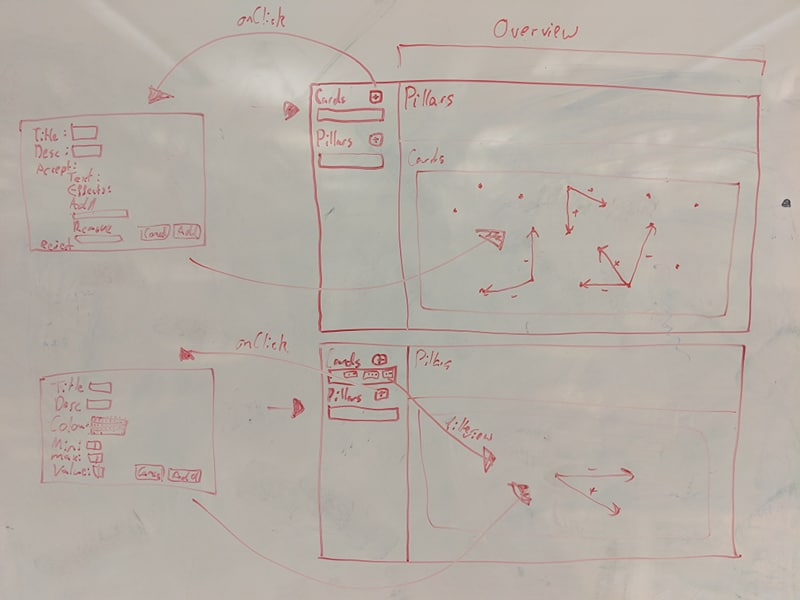
\includegraphics[width=0.36\textwidth]{./images/design/game_maker_drawing.png}
	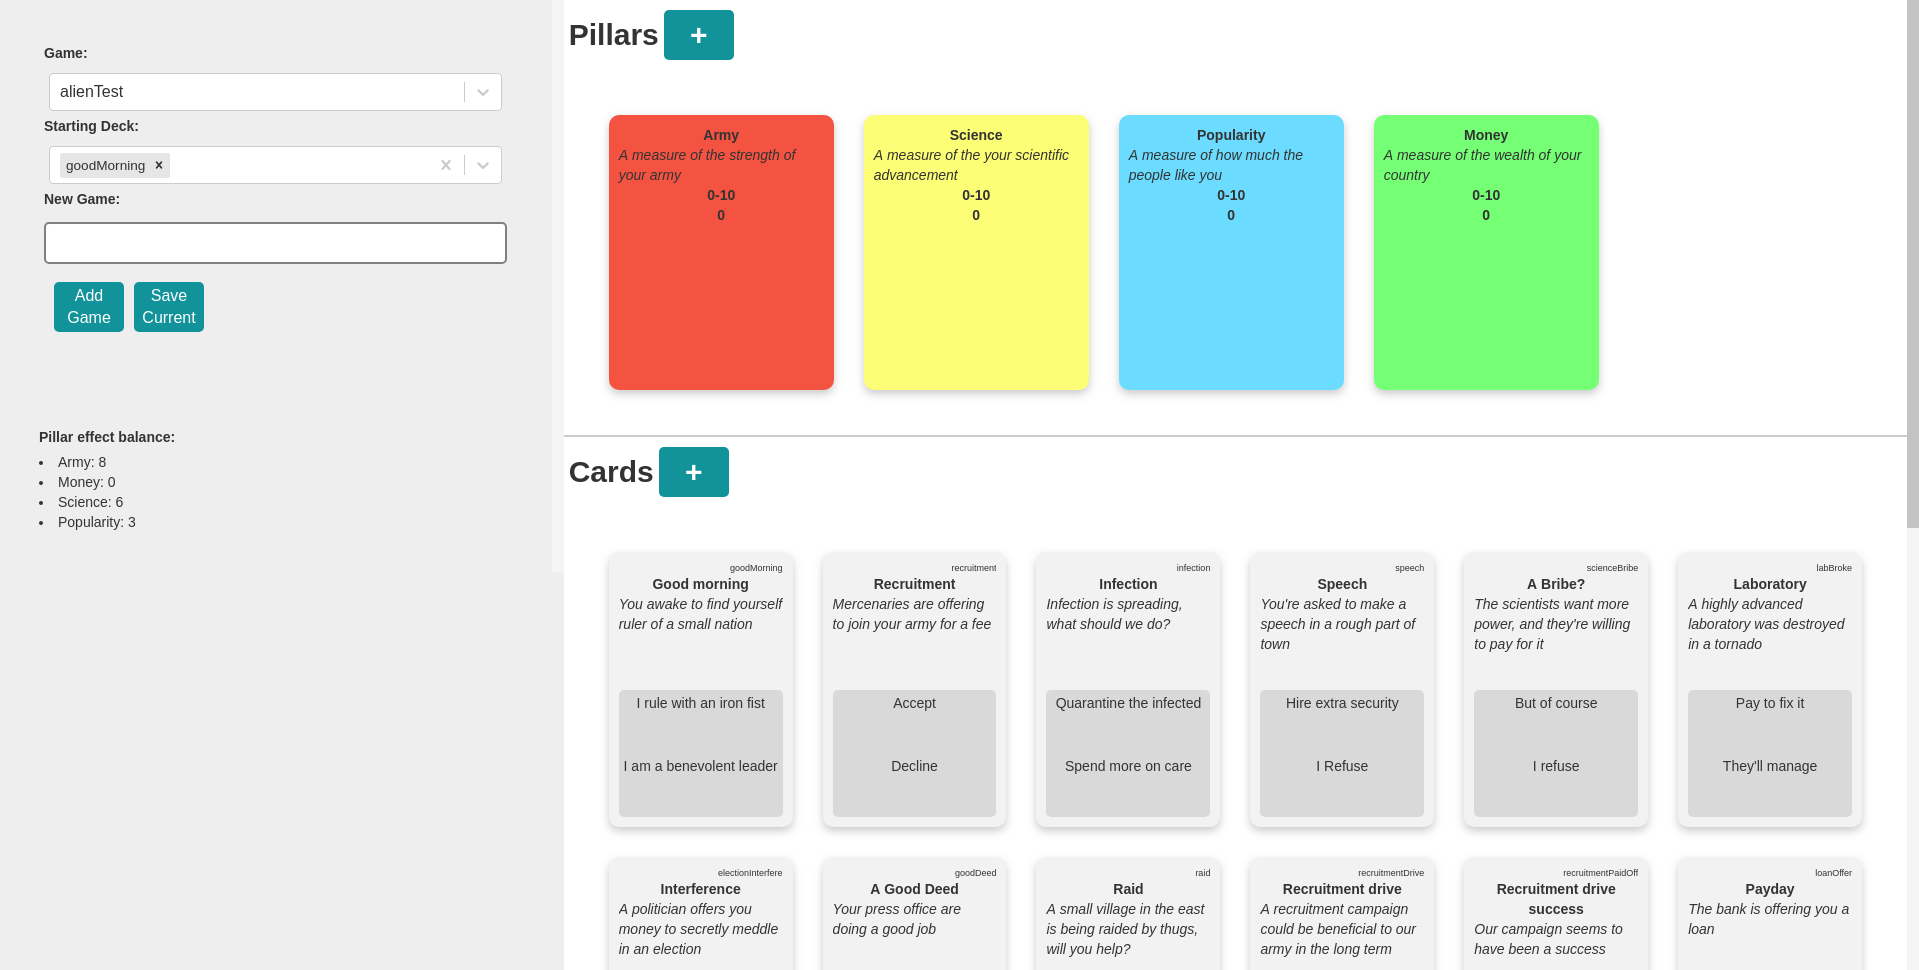
\includegraphics[width=0.54\textwidth]{./images/design/game_maker.png}
	\caption{Comparison between initial and final designs for the game maker. Shown is the example game I created for demonstration purposes.}
	\label{fig:game_maker}
\end{figure}

In the section on the right, the user can see the game pillars and cards that they have created. This side is scrollable, while the left section remains in view. If the details of a card are too large for the view, the text fades out. The card view can be expanded by hovering over it, as seen in figure \ref{fig:expand} - when this is done, other cards shrink and move to allow the extra space. New cards and pillars can be added with the large \c{+} buttons by the headers, while existing ones can be edited by clicking on them. Both of these options opens the edit view on the left section.

\begin{figure}[!h]
	\centering
	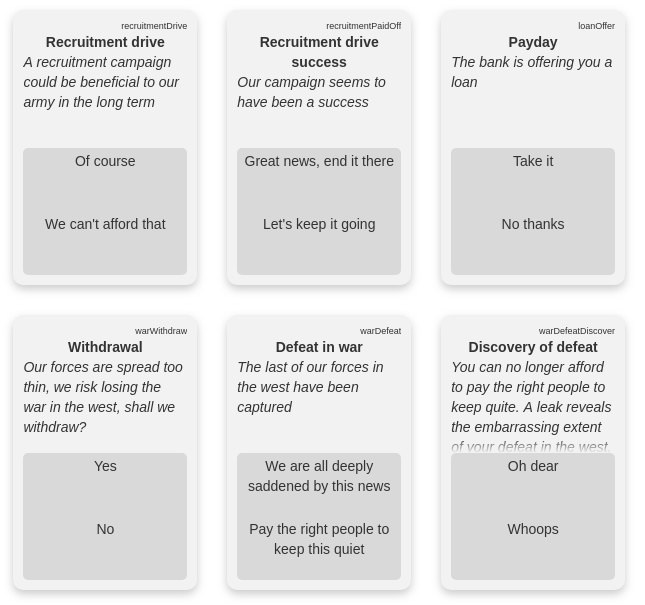
\includegraphics[width=0.45\textwidth]{./images/design/cards_not_expanded.png}
	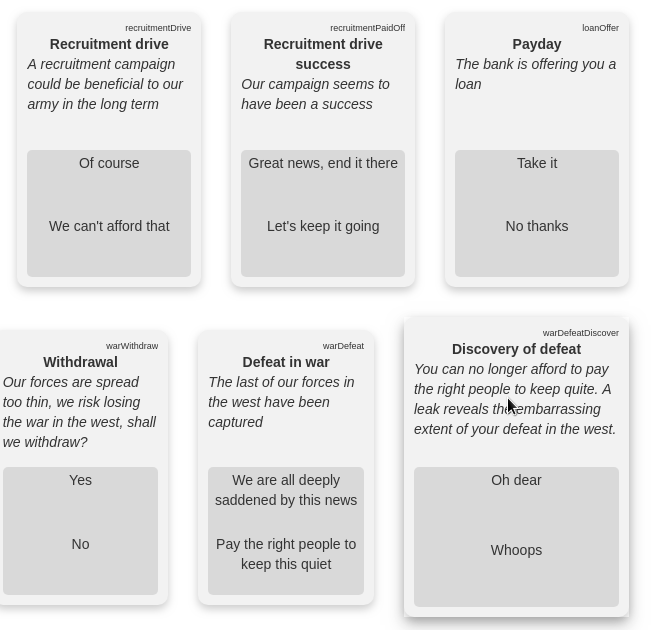
\includegraphics[width=0.45\textwidth]{./images/design/cards_expanded.png}
	\caption{Demonstration of hover expanded view (note that the full text is cut off on the left, readable on the right)}
	\label{fig:expand}
\end{figure}

The left section provides contextual menus. When no pillar or card is selected, it provides high-level functionality, such as saving, switching, or creating new game definitions. Also present here is starting deck selection, game balance information and any warnings.

The pillar effect balance provides the admin user with an idea of how balanced their game is in its current state. This is done by summing all of the effects that are applied to each pillar for any given response to all cards. This acts as an indicator of how well a user is likely to do if they randomly pick their responses. The higher the balance values, easier the game.

Warnings appear when a card has no chance of being added to the game. This means that a card has been created, but it is neither in the starting deck, nor is it added by any other card. This is only a shallow check - if card A is added by another card B, which itself is never added, the warning will only appear for card B. I consider this acceptable, as once card B is added or deleted, the situation will be resolved.

\begin{figure}[!h]
	\centering
	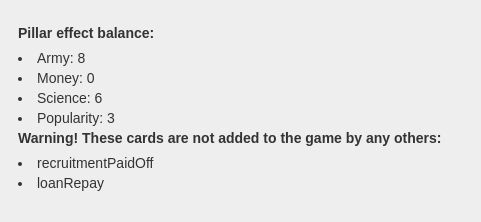
\includegraphics[width=0.6\textwidth]{./images/design/info.png}
	\caption{Info on left panel. Note the two warnings, which appeared on removing \c{recruitmentPaidOff} and \c{loanRepay} from all `cards added' lists}
	\label{fig:info}
\end{figure}

When editing a card, a live preview can be seen at the bottom of the panel, along with buttons to cancel changes, delete, or submit the card. When editing the consequences, adding and removing cards is done through a dropdown list, which allows multiple cards to be selected.

\begin{figure}[!h]
	\centering
	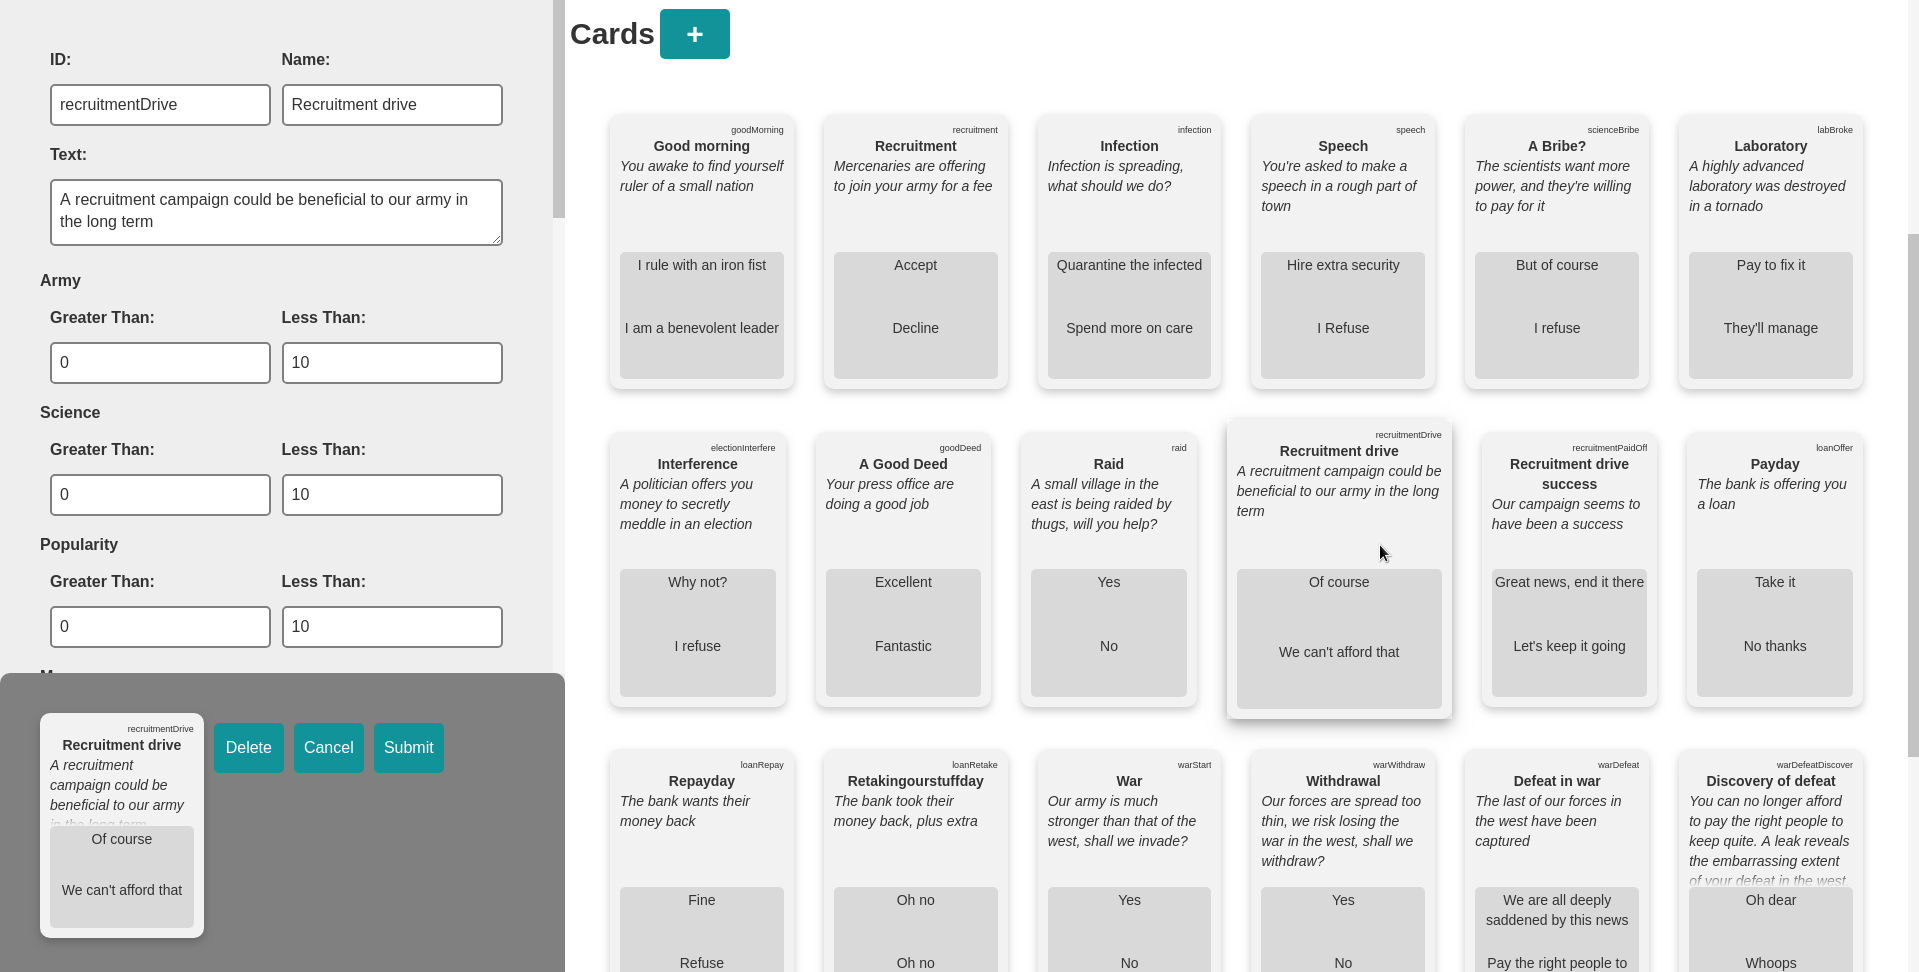
\includegraphics[width=1.0\textwidth]{./images/design/card_edit.png}
	\caption{Card editing view, reached by selecting a card by clicking it.}
	\label{fig:card_edit}
\end{figure}

\begin{figure}[!h]
	\centering
	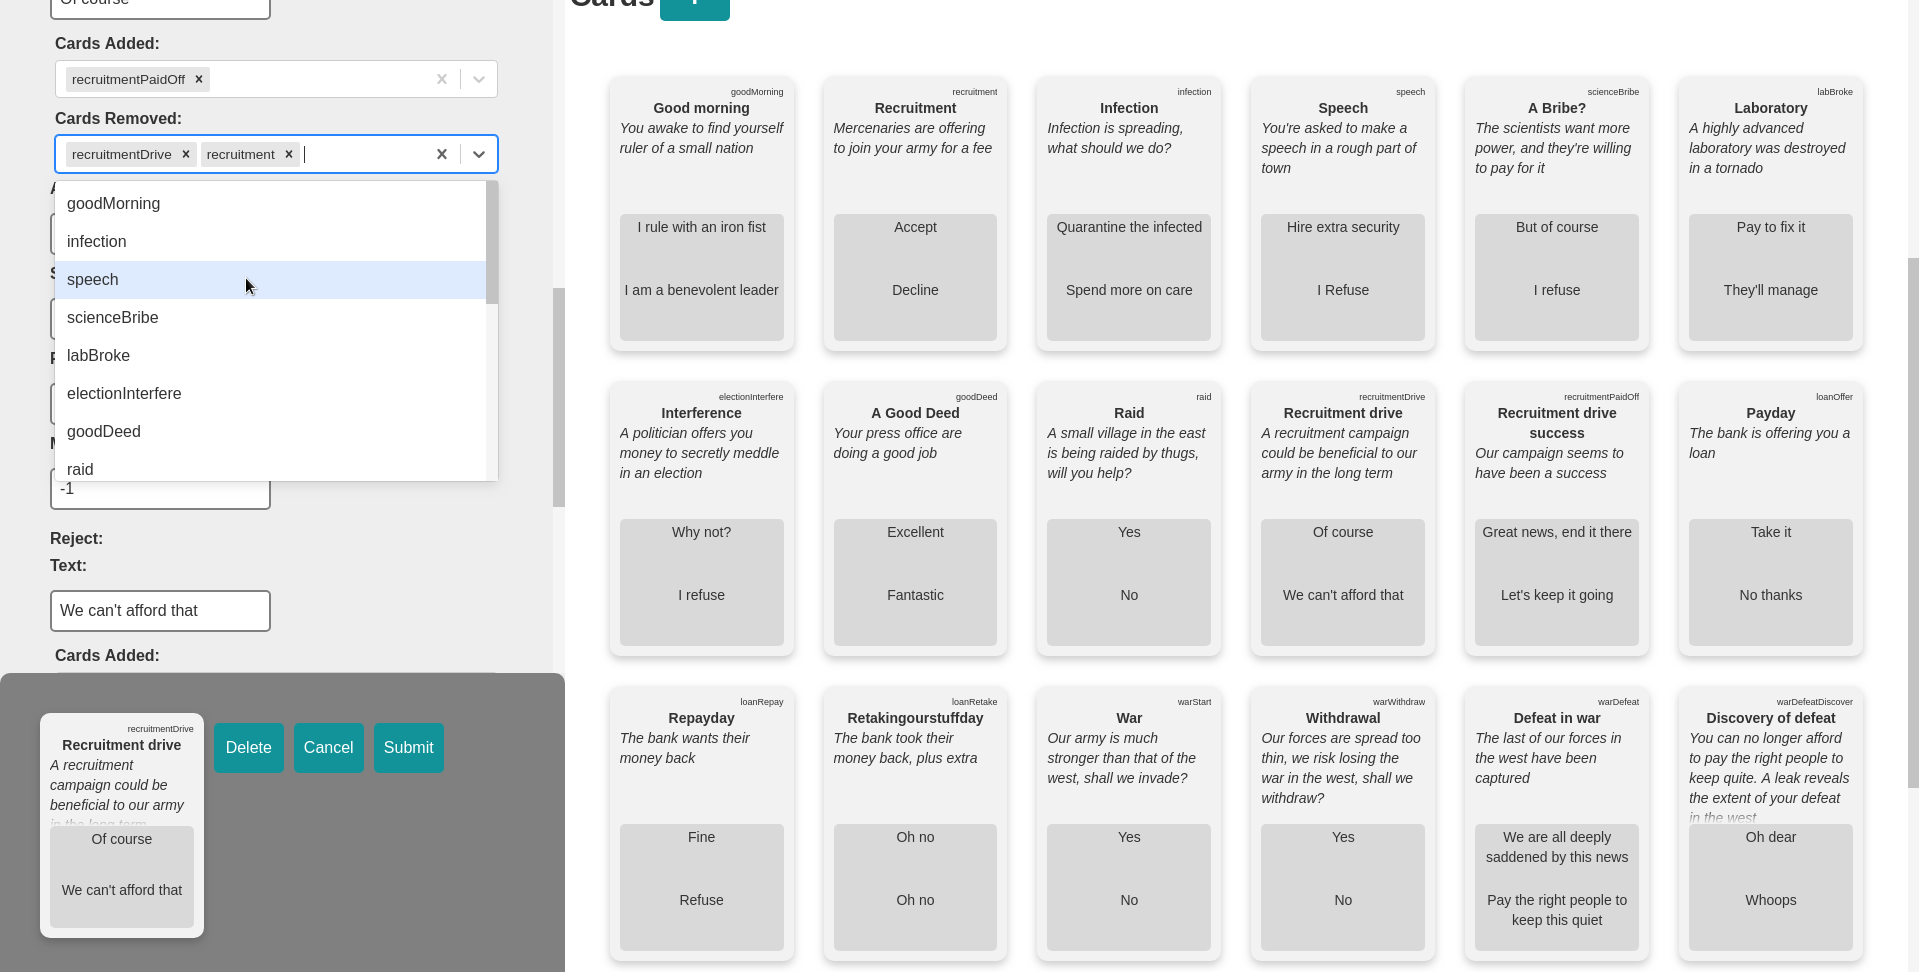
\includegraphics[width=1.0\textwidth]{./images/design/add_card.png}
	\caption{Dropdown showing all other cards that can be added or removed}
	\label{fig:add_card}
\end{figure}

Figure \ref{fig:pillar_edit} shows the pillar editing menu, which is very similar to the card editing view. The colour of the pillar can be entered as a hex value, which is immediately reflected in the preview below.

\begin{figure}[!h]
	\centering
	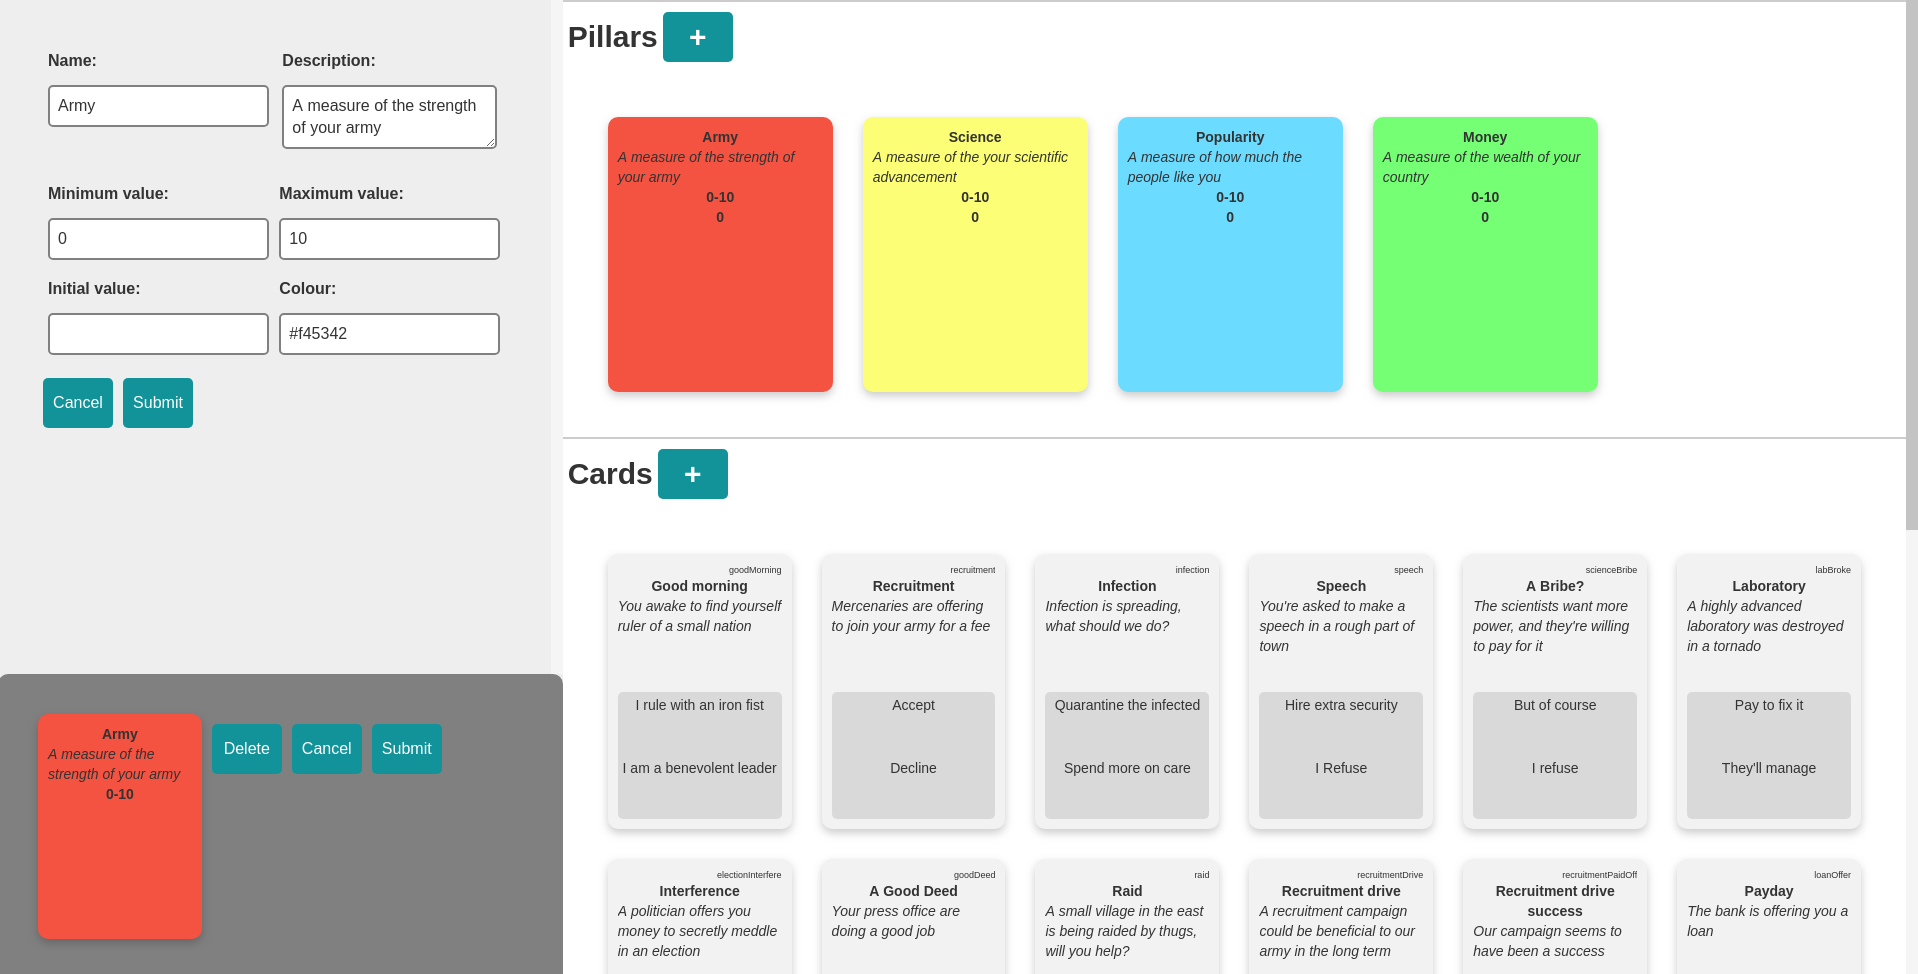
\includegraphics[width=1.0\textwidth]{./images/design/pillar_edit.png}
	\caption{Pillar editing view}
	\label{fig:pillar_edit}
\end{figure}

Clicking \c{Save Current} will save the updated game definition to the database, and it can then be played from the game UI by entering the correct game ID.

\subsubsection{Visualisation}
\todo[inline]{Discuss export}

The visualisation screen took a similar shape to the game maker, with data selection and filtering happening in a left panel while the visualisations are updated on the right.
It is possible to filter results to be visualised by pillar values. This limits the data shown only to cards that appeared while pillar values match the specified criteria The visualisations I chose to show are as follows:
\begin{itemize}
	\item Accept/Reject balance

	      This is a horizontal bar chart showing the proportion of players that choose one option over the other for a given set of cards. Each card has a value between -1 and 1, where -1 indicates that players choose the reject option every time, while 1 indicates accept is chosen every time.

	\item Total times drawn

	      This is a vertical bar chart showing the total number of times each card has been drawn and responded to.

	\item Pillar average

	      This shows the average pillar levels over all turns.
\end{itemize}

The intention of these visualisations is to allow a user to `play' with the data. The live updating charts allow the user to rapidly identify relationships, for example between pillar levels and accept/reject balance.

\begin{figure}[!h]
	\centering
	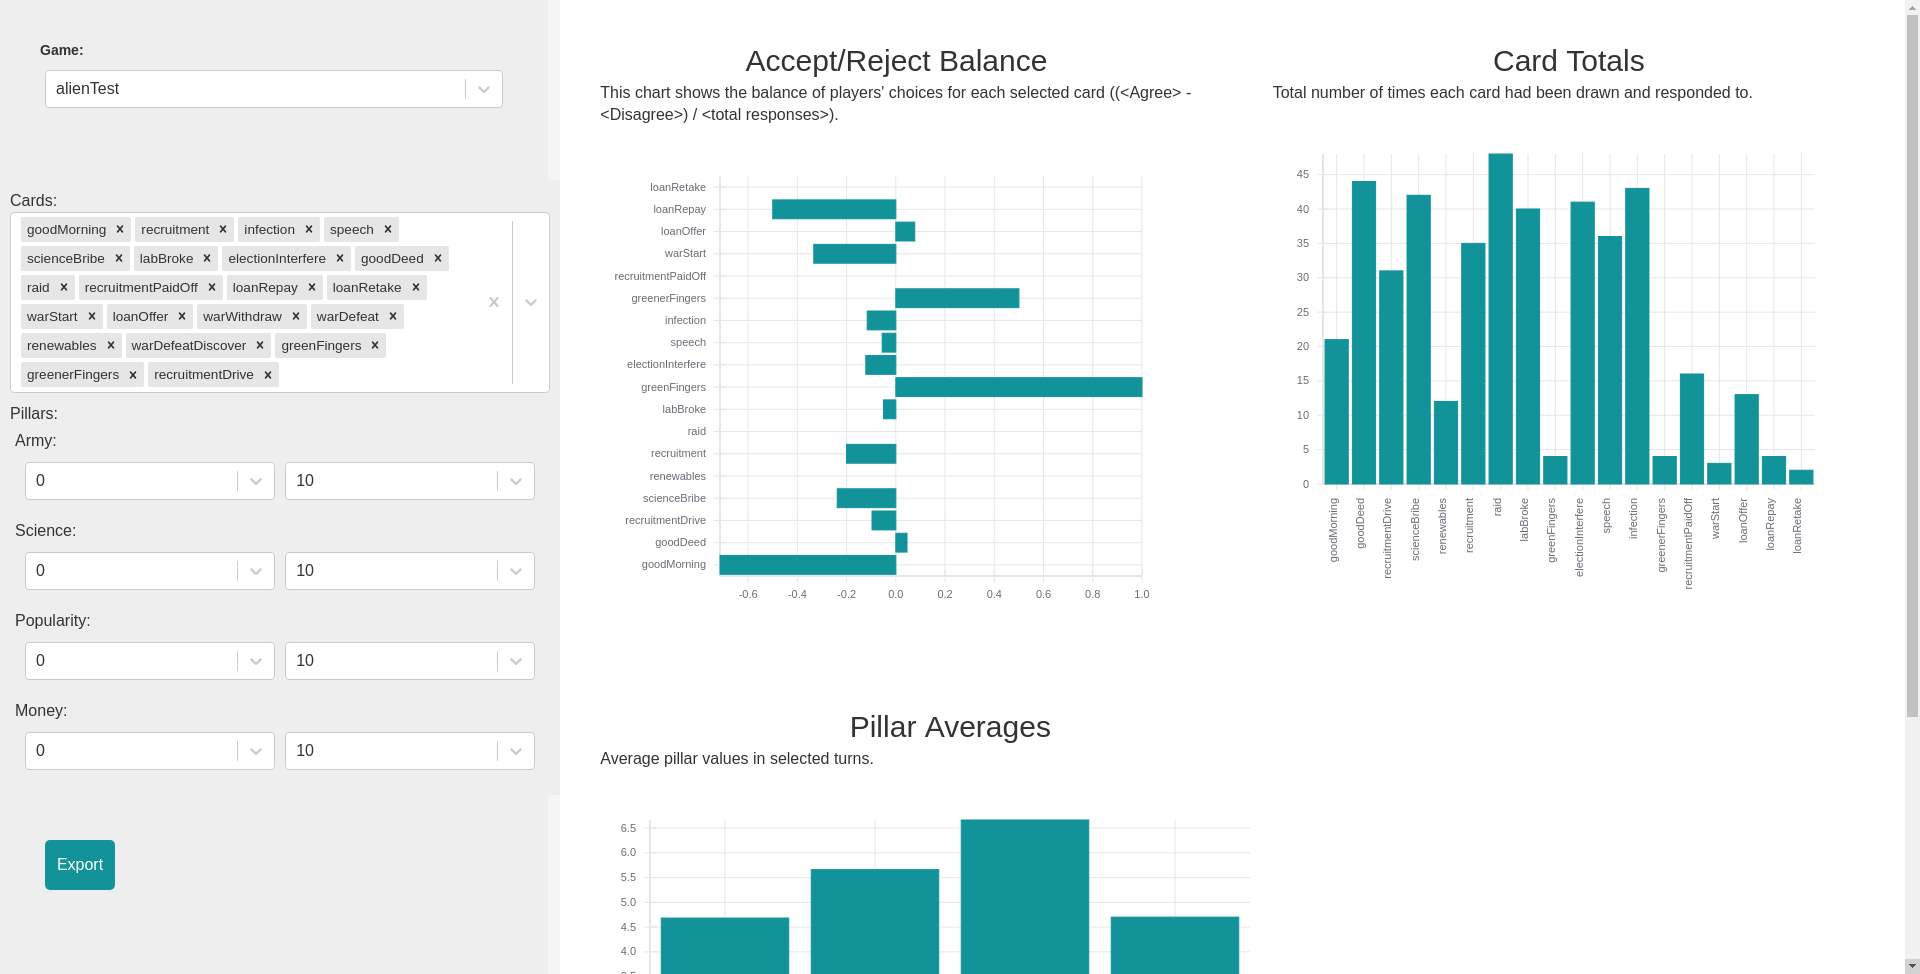
\includegraphics[width=0.45\textwidth]{./images/design/visualisation.png}
	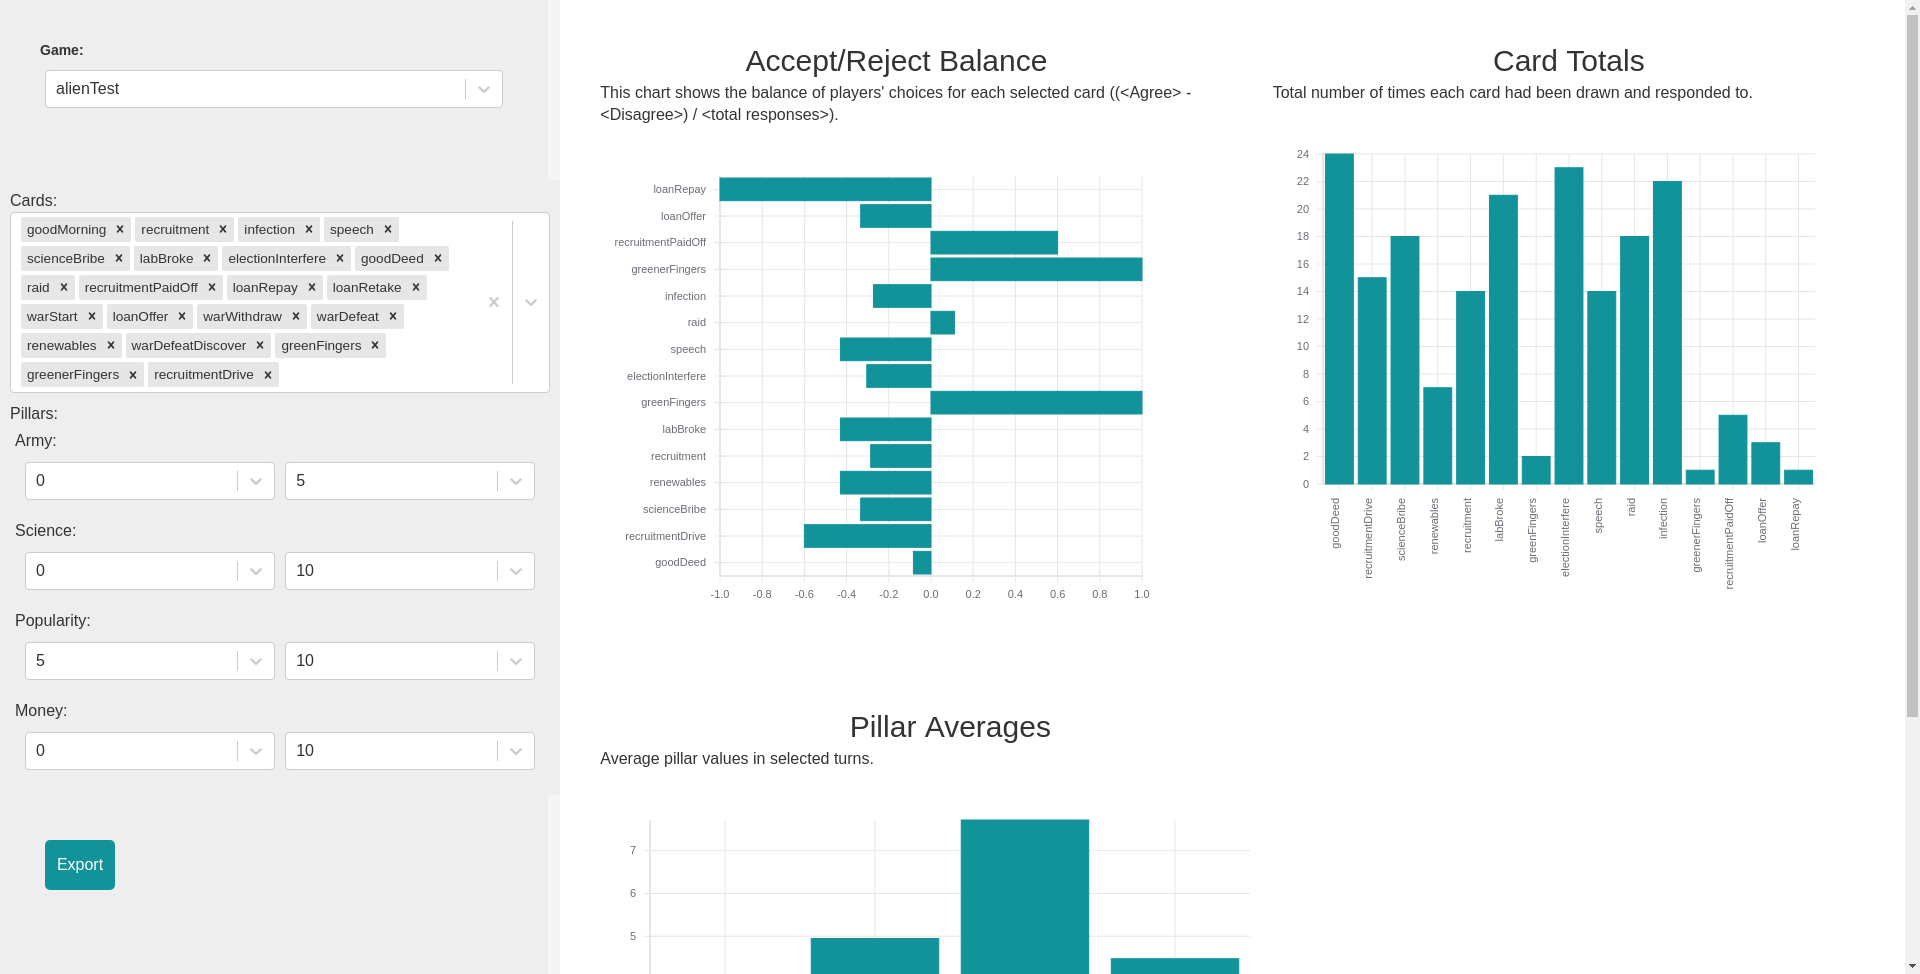
\includegraphics[width=0.45\textwidth]{./images/design/visualisation_filter.png}
	\caption{Visualisation screen effects of filtering data by cards and pillar values. This example filters responses to cards during turns where the player's \c{Army} was between 0 and 5, and their \c{Popularity} was between 5 and 10.}
	\label{fig:visualisation}
\end{figure}

The other function this page offers is the ability to export data to CSV. This effectively repackages the database as a csv file, where each row represents the turn of a user. Individual games are uniquely identified by sets of rows with the same user id and game id.

\section{Frontend}
When using Redux, one of the first design decisions that must be made is the structure of the Redux store. This is the JavaScript object that holds the page's state. Figures \ref{fig:store_shape} and \ref{fig:card_example} show a visual representation of the store for the game site. The game logic runs client-side, so to enable this, the entire game definition is requested from the database server once the player requests to play it. Depending on the use case, this could be considered a downside as technically a player could `cheat' the game through using console commands. This choice did however greatly simplify the API between the client and sever, as once the game has begun, the client only needs to send the outcome of each turn.

\begin{figure}[!h]
	\centering
	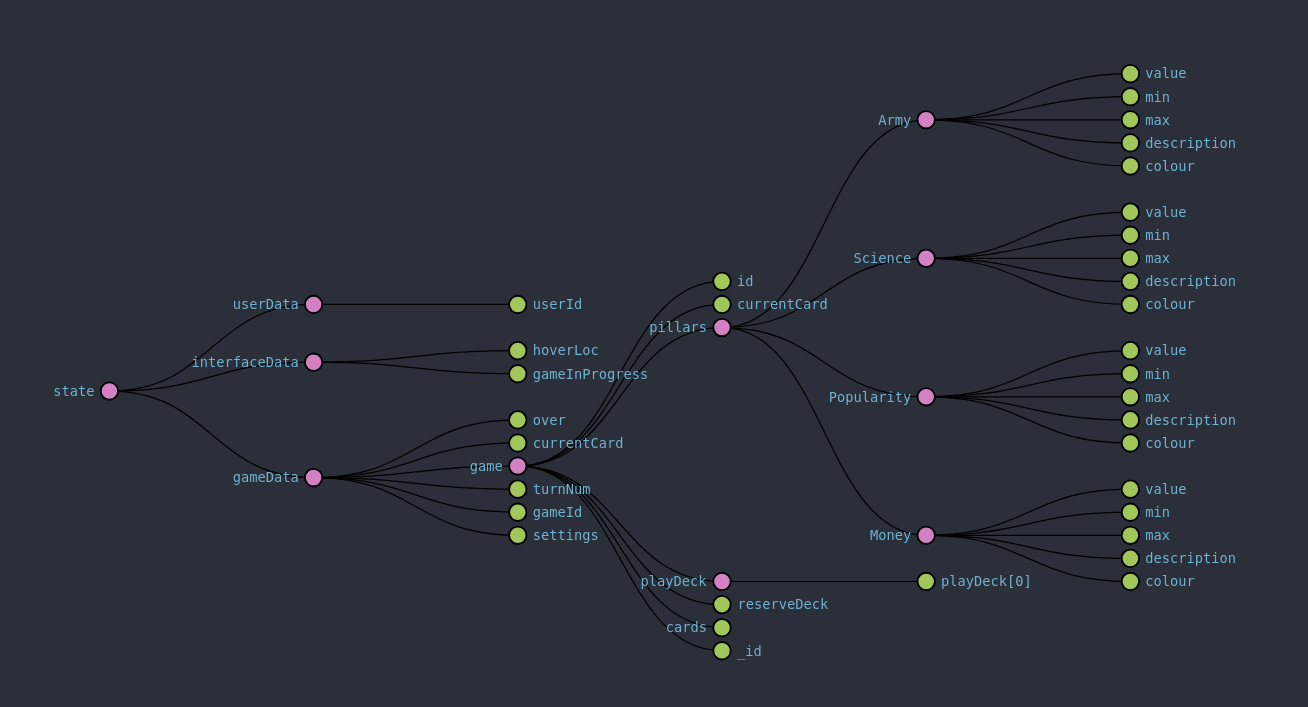
\includegraphics[width=1.0\textwidth]{./images/design/store_shape.png}
	\caption{Redux store object structure. Note that the pillars (Army, Science, Popularity, Money) are game definition dependent. Cards object is omitted due to large size.}
	\label{fig:store_shape}
\end{figure}

\begin{figure}[!h]
	\centering
	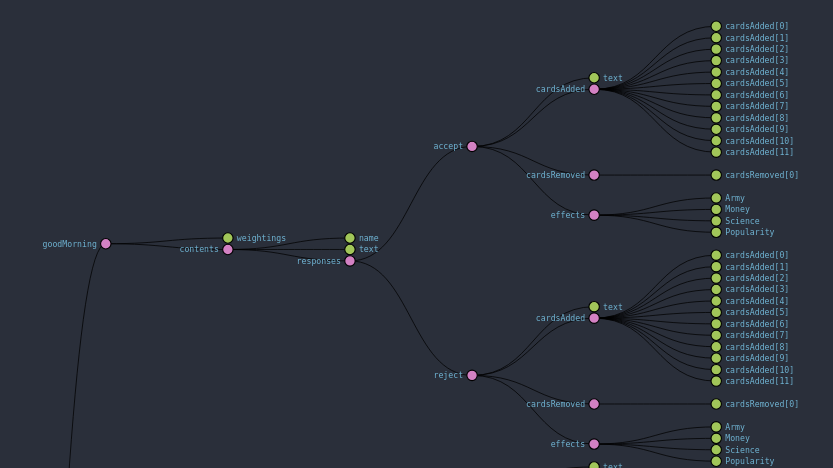
\includegraphics[width=1.0\textwidth]{./images/design/card_example.png}
	\caption{Example of a card object in the store. This is a starting card that adds many other cards to the game no matter which option is chosen.}
	\label{fig:card_example}
\end{figure}

\section{Backend}
Access to the database is provided through a backend server, which exposes a RESTful \cite{REST} API. This is a lightweight server that directly accesses and modifies the databases, of which there are two. One database stores game definitions, while the other stores user turn data.
The brief API documentation 
